\chapter{Expertsystemen}
\begin{itemize}
	\item Kennis van een \textbf{echte expert} overnemen in een programma.
	\item De \textbf{gebruiker} moet ook enigszins kennis hebben. Hij moet de conclusies begrijpen en toepassen.
	\item \textbf{MYCIN}: een expertsysteem om te helpen bij de diagnose van bepaalde besmettelijke bloedziekten.
	\begin{itemize}
		\item Is in staat om een betere diagnose te stellen dan een arts die geen expert is in het gebied.
		\item De gebruiker moet wel een arts zijn die de diagnose begrijpt.
	\end{itemize}
	\item Een expertsysteem maakt gebruik van \textbf{vuistregels}, waarop later nog \textbf{verfijningen} ingevoerd worden:
	\begin{enumerate}
		\item werken met \textbf{onzekere conclusies}. Dit wordt ingevoerd om contradicties te behandelen indien deze voorkomen.
		\item De invoering van \textbf{frames}. Zorgt voor een betere orderning voor grote hoeveelheden kennis.
	\end{enumerate}
\end{itemize}
\section{Eenvoudige systemen}
\begin{itemize}
	\item Een expertsysteem bestaat uit \underline{twee hoofdcomponenten}
	\begin{enumerate}
		\item Een \textbf{kennisbank}:
		\begin{itemize}
			\item bevat \textbf{feiten}: dit zijn uitspraken die waar zijn.
			\item bevat \textbf{regels}: dit heeft de vorm \textbf{als$<$premisse$>$dan$<$conclusie$>$}
			\regel{AS=rond \textbf{en} MATERIAAL=staal}{SMERING=olie}
		\end{itemize}
		\item Een \textbf{afleidingssysteem}:
		\begin{itemize}
			\item Elk probleem bestaat uit begingegevens en een doel.
			\item Deze gegevens vormen een lijst van feiten die gekend zijn.
			\item Het doel is ook een lijst van uitspraken.
			\item Het doel is bereikt als één uitspraak uit de lijst is afgeleid uit de gegevens.
		\end{itemize}
	\end{enumerate}
	\item Het afleidingssysteem kan op \underline{twee manieren} werken.
	\begin{itemize}
		\item \textbf{Forward chaining:}
		\begin{itemize}
			\item Kan in $O(g)$, met $g$ de grootte van de regelbank.
			\item Twee gegevensstructuren:
			\begin{itemize}
				\item \textbf{LijstMetRegels($u$)} die voor elke uitspraak $u$ bijhoudt in welke regels ze in de premisse voorkomt.
				\item \textbf{Premisseteller($r$)} die voor elke regel $r$ bijhoudt hoeveel uitspraken in de premisse nog niet gevalideerd zijn.
			\end{itemize}
			\item Werking:
			\begin{enumerate}
				\item Initialiseer de gegevensverzameling en de doelverzameling.
				\item Voor elke regel $r$, initialiseer \textit{Premisseteller($r$)}
				 op het aantal uitspraken in de premisse.
				\item Zolang de gegevensverzameling en het doel geen gemeenschappelijk element bevatten, en de gegevensverzameling niet leeg is:
				\begin{enumerate}
					\item Neem een uitspraak $u$ uit de gegevensverzameling.
					\item Voor elke regel $r$ in \textit{LijstMetRegels($r$)}, verminder \textit{Premisseteller($r$)}. Als deze daardoor nul wordt, zet elke uitspraak uit de conclusie die nog niet behandeld is in de gegevensverzameling.
				\end{enumerate}
				\item Deel het resultaat mee aan de gebruiker.
			\end{enumerate}
			\item \underline{Voorbeeld:}
			\begin{itemize}
				\item Stel volgende regelbank:
				
				\noindent\fbox{%
					\parbox{\linewidth}{%
						\regel{$X$ kwettert en $X$ zingt}{$X$ is een kanarie}
						\regel{$X$ kwaakt en $X$ eet vliegen}{Dan $X$ is een kikker}
						\regel{$X$ is een kikker}{$X$ is groen}
						\regel{$X$ is een kanarie}{$X$ is geel}
					}%
				}


				\item Stel nu dat we een huisdier hebben, Fritz,  en er zijn twee dingen bekend over hem: hij kwaakt en eet vliegen. We willen nu de kleur weten.
				\item Fritz wordt gesubstitueerd voor $X$ in regel 1, maar hij voldoet niet aan de premisse. Hij wordt nu gesubstitueerd voor $X$ in regel 2, zodat er besloten wordt dat hij een kikker is. Dit wordt dan toegevoegd aan de gegevens. We weten nu dat Fritz kwaakt, dat hij vliegen eet en dat hij een kikker is.
				\item Fritz kan nu gesubstitueerd worden in regel 3, zodat er besloten wordt dat hij groen is.
			\end{itemize}
			\item Forward Chaining werkt van links naar rechts, startend vanaf de gekende feiten om tot een conclusie te komen.
			\alert In het algoritme kunnen regels toegepast worden die uiteindelijk niet bijdragen tot de oplossing. Men probeert dit efficiënter op te lossen met backwards chaining.
		\end{itemize}
		\item \textbf{Backward chaining:}
		\begin{itemize}
			\item Kan in $O(g)$, met $g$ de grootte van de regelbank.
			\item Werking:
			\begin{enumerate}
				\item[$A.$] Behandeling voor een regel waarbij alle uitspraken uit de premisse gegevens zijn:
				\begin{enumerate}
					\item[$A1.$] Voeg alle uitspraken uit de conclusie toe aan de gegevens.
					\item[$A2$] Voor alle tussenregels voor wie, op deze manier, alle uitspraken uit de premisse gegevens zijn geworden, behandel ze volgens $A$.
					\item[$A3.$] Verwijder de regel uit de regelbank of uit de verzameling tussenregels.
				\end{enumerate}
				\item[$B.$] Behandeling voor een regel waarbij niet alle uitspraken uit de premisse gegevens zijn:
				\begin{enumerate}
					\item[$B1.$] Voeg alle uitspraken uit de premisse die geen gegevens zijn toe aan de tussendoelverzameling.
					\item[$B2.$] Verwijder de regel uit de regelbank en voeg hem toe aan de tussenregels.
				\end{enumerate}
				\item[$C.$] Oplossingsalgoritme:
				\begin{enumerate}
					\item Initialiseer de gegevensverzameling en doelverzameling. Initialiseer ook de verzamelingen van tussendoelen en tussenregels: deze zijn leeg.
					\item Zolang er geen resultaat is gevonden, en er een regel is uit de regelbank wiens conclusie een doel of een tussendoel bevat, doe het volgende:
					\begin{enumerate}
						\item Neem zo een regel.
						\item Als alle uitspraken uit de premisse gegevens zijn, behandel volgens $A$, anders volgende $B$.
					\end{enumerate}
				\end{enumerate}
			\end{enumerate}
			\item \underline{Voorbeeld:}
			\begin{itemize}
				\item Veronderstel dezelfde regelbank als bij forward chaining.
				\item Stel nu dat we een huisdier hebben, Fritz,  en er zijn twee dingen bekend over hem: hij kwaakt en eet vliegen. We willen nu de kleur weten.
				\item Fritz wordt gesubstitueerd voor $X$ in regel 3. Men moet dan bewijzen dat Frits een kikker is.
			\end{itemize}
		\end{itemize}
	\end{itemize}
\end{itemize}
\section{De constructie van een expertsysteem}
\begin{itemize}
	\item \underline{Twee soorten kennis nodig:}
	\begin{itemize}
		\item Kennis over het probleemgebied. Experten in het toepassingsgebied weten hoe ze problemen moeten oplossen, maar kunnen deze kennis niet vertalen in de vorm die een expertsysteem nodig heeft.
		\item Kennis over expertsystemen. Een team die de kennis van de experten kan filteren en omvormen naar de juiste vorm. 
	\end{itemize}
\end{itemize}
\section{Onzekerheid}
\begin{itemize}
	\item De relatie tussen premisse en conclusie van een regel is niet altijd zeker.
	\item \underline{Voorbeeld:}
	\begin{itemize}
		\item Een expertsysteem dat de oorzaak zoekt van problemen in een computer. Dit systeem kan een reparateur begeleiden die een defecte computer moet repareren.
		\item De reparateur moet melden wat de symptomen zijn. Het systeem moet de actie bepalen die moet ondernomen worden om het probleem op te lossen. Mogelijke regels zijn bijvoorbeeld:
		\regel{SYMPTOOM=computer doet niets bij opstarten}{PROBLEEM=voeding defect}
		\regel{SYMPTOOM=voeding defect}{PROBLEEM=vervang voeding}

		
		\item Maar soms kan een probleem meerdere oorzaken hebben, waarbij sommige meer waarschijnlijkheid hebben dan anderen:
		\regel{PROBLEEM=bootloader hangt}{OORZAAK=schijf defect \textbf{of} OORZAAK=bootloaderinstallatie \textbf{of} ...}

		
		\item Er wordt dan een numerieke factor toegekend, die de waarschijnlijkheid aanduidt. 
		
		\item \textbf{Hoe wordt de numerieke waarde bepaalt?}
		\begin{enumerate}
			\item Vage verzamelingen: \textbf{Niet te kennen}.
			\item Bayesiaans redeneren: 
			\begin{itemize}
				\item Stel volgende regels:
				\regel{het regent op dag x}{is de kans dat het op dag x + 1 regent 0,8}
				\regel{het niet regent op dag x}{is de kans dat het op dag x + 1 regent 0,3}

				\item Statistisch redeneren kan toegepast worden in expertsystemen als er voldoende statistische informatie is:
				\begin{itemize}
					\item De kans dat het morgen en overmorgen regent: $0,8 \times 0,8 = 0,64$.
					\item Da kans dat het morgen niet regent, maar overmorgen wel: $0,2 \times 0,3 = 0,06$.
				\end{itemize}
				\item Stel dat we nu twee uitspraken $a$ en $b$ hebben met $p(a) = 0,8$ en $p(b) = 0,2$.
				\item Wat is de kans op $p(a\; \hbox{\textbf{en}}\;b)$? Deze waarde kan tussen 0 en 0,2 liggen. 
				
				Als $a = $ het regent morgen en $b = $ het regent niet morgen, dan is $p(a\; \hbox{\textbf{en}}\;b) = 0$. 
				
				Als $a = $ het regent morgen en $b = $ het regent morgenochtend, dan is $p(a\; \hbox{\textbf{en}}\;b) = 0,2$
				
				\alert Bayesiaans redeneren is geen aangewezen methode.
			\end{itemize}
			\item Theorie van zekerheidsfactoren:
			\begin{itemize}
				\item Er wordt een zekerheidsfactor berekent op basis van woorden die een expert uitdrukt:
				\begin{table}[h]
					\centering
					\begin{tabular}{| l | c |}
						\hline 
						Term & zekerheidsfactor \\
						\hline 
						zeker niet & -1,0 \\
						bijna zeker niet & -0,8 \\
						waarschijnlijk niet & -0,6 \\
						misschien niet & -0,2 tot +0,2 \\
						misschien & +0,4 \\
						waarschijnlijk & +0,6 \\
						bijna zeker & +0,8 \\
						zeker & +1,0 \\
						\hline
					\end{tabular}
				\end{table}
			
				\item Voor een uitspraak $a$ wordt de zekerheidsfactor van die uitspraak $z(a)$. Hierbij geldt $z(a) = -z(\neg a)$.
				
				\item Hoe berekenen van de zekerheid van een conclusie als de premisse van een regel zelf onzeker is?
				
				\begin{itemize}
					
					\item[] \noindent\fbox{%
						\parbox{\linewidth}{%
							\begin{equation*}
							\begin{split}
							& \hbox{\textbf{als} b} \\
							& \hbox{\textbf{dan} a \qquad (x)}  
							\end{split}
							\end{equation*}
								$$z(a) = z(b) \times x$$
						}%
					}
		
					\item[]
					\noindent\fbox{%
						\parbox{\linewidth}{%
						\begin{equation*}
						\begin{split}
						& \hbox{\textbf{als} b \textbf{en} c \textbf{en} d} \\
						& \hbox{\textbf{dan} a \qquad (x)}  
						\end{split}
						\end{equation*}
					$$z(b\;\hbox{\textbf{en}}\;c\; \hbox{\textbf{en}}\;d) = \min(z(b), z(c), z(d)) \times x$$
						}%
					}
					
					
				
					\item[] \noindent\fbox{%
						\parbox{\linewidth}{%
						\begin{equation*}
						\begin{split}
						& \hbox{\textbf{als} e} \\
						& \hbox{\textbf{dan} a \qquad (x)}  
						\\[3ex]
						& \hbox{\textbf{als} f} \\
						& \hbox{\textbf{dan} a \qquad (y)}  
						\end{split}
						\end{equation*}
						$$z_1 = z(e) \times x,\qquad z_2 = z(f) \times y$$
						$$z(a) = \frac{z_1 + z_2}{1 - \min(|z_1|, |z_2|)}$$
						
							
						}%
					} 
		
				\end{itemize}
			\end{itemize}
		\end{enumerate}	
	\end{itemize}
\end{itemize}

\section{Frames en regelschema's}
\begin{itemize}
	\item Noodzaak om kennis in te delen.
	\item Een \textbf{frame} kan vergeleken worden met een klasse uit object georiënteerde programeertalen.
	\item Komt uit de theorie van \textbf{semantische netten}.
	\begin{figure}[ht]
		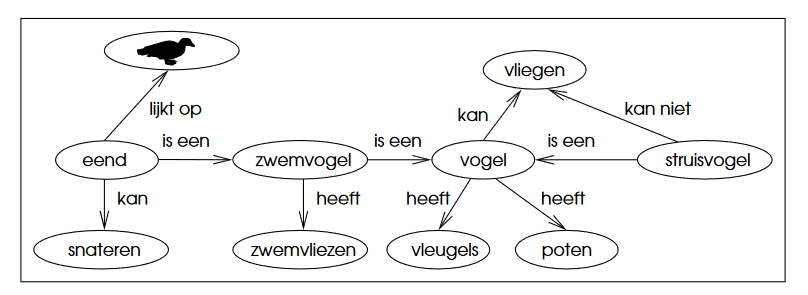
\includegraphics[width=\textwidth]{semantisch_net}
		\caption{Een semantisch net.}
	\end{figure}
	\begin{itemize}
		\item Een semantisch netwerk bestaat uit een gelabelde gerichte multigraaf.
		\item Elke knoop is een begrip, en elk begrip is verbonden met andere begrippen.
	\end{itemize}
	\item Opzoeken van informatie:
	\begin{itemize}
		\item \textit{Kan een eend snateren?} Vanuit 'eend' wordt de 'kan'-relatie naar 'snateren' genomen. Het antwoord is 'ja'.
		\item \textit{Heeft een eend zwemvliezen?} Via de 'is een'-relatie weet men dat een eend een zwemvogel is. De zwemvogel bevat een 'heeft'-relatie naar 'zwemvliezen'. Het antwoord is 'ja'.
		\item \textit{Heeft een eend vleugels?} Via de twee 'is een'-relaties weet men dat een eend een vogel is. Een vogel bevat een 'heeft'-relatie naar 'vleugels'. Het antwoord is 'ja'.
		\item \textit{Eet een eend sla?} Na het netwerk te hebben afgezocht is er geen verband tussen sla en eenden gevonden.
		
	\end{itemize}
	\item Twee regels om informatie op te zoeken:
	\begin{enumerate}
		\item Volg de takken waarvan de naam in de vraag staat.
		\item Volg de takken met 'is een' als naam. Deze zorgt ervoor dat het probleem veralgemeend wordt (eend wordt zwemvogel en dan vogel), maar het wordt enkel gebruikt als er geen andere informatie meer beschikbaar is via andere relaties.
	\end{enumerate}
	\item \textit{Kan een struisvogel vliegen?}  We vinden informatie met de 'kan niet'-relatie zodat het antwoord 'nee' is. 
	\alert Het net bevat enkel informatie en geen regels voor de verwerking ervan.
	\item Frames versus objectgeoriënteerd programmeren:
	\begin{enumerate}
		\item Ze hebben beiden een hiërarchisch systeem dat gebruik maakt van (geen meervoudige) overerving.
		\item In een semantisch net wordt er geen onderscheid gemaakt tussen klassen en objecten.
	\end{enumerate}
	
\end{itemize}